147. \begin{figure}[ht!]
\center{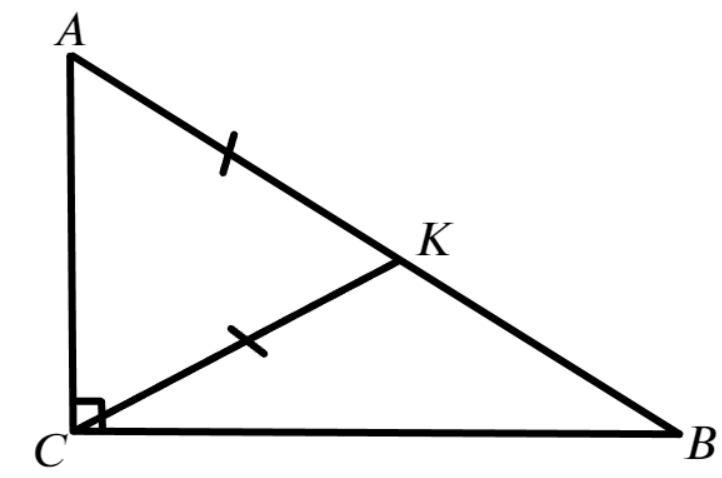
\includegraphics[scale=0.35]{g7-147.png}}
\end{figure}\\
Треугольник $AKC$ является равнобедренным, значит $\angle A=\angle ACK.$ Но тогда $\angle KCB=90^\circ-\angle ACK=90^\circ-\angle A=\angle B$ и треугольник $CKB$ также является равнобедренным, поэтому $KB=KC=6.$\\
